\subsection{Escalas de tiempo}

\begin{frame}[t]
\frametitle{\subsecname}

Una escala de tiempo es un conjunto cerrado $\mathds{T}$ bajo la topología estándar sobre $\mathds{R}$.

Se define el operador salto posterior $\sigma\colon\mathds{t}\rightarrow\mathds{T}$ por \[ \sigma\left(T\right)\coloneqq\inf\left\{z\in\mathds{T}:z>t\right\} \]

la granicidad $\mu\colon\mathds{T}\rightarrow\mathds{R}$ por \[ \mu\left(t\right)=\sigma\left(t\right)-t \] y función granicidad minimal $\mu_{\ast}\colon\mathds{T}\rightarrow\mathds{R}$ por \[ \mu_{\ast}\left(s\right)=\inf_{\tau\in\left[s,\infty\right)\cap\mathds{T}}\mu\left(t\right). \]

Una función $f\colon\mathds{T}\rightarrow\mathds{C}$ es llamada $\Delta$--diferenciable si para cualquier $\varepsilon>0$ existe $\delta>0$ tal que para todo $s\in\left(t-\delta,t+\delta\right)\cap\mathds{T}$ y existe un número $f^{\Delta}\left(t\right)$ tal que \[ |\left[f\left(\sigma\left(s\right)\right)-f\left(s\right)\right]f^{\Delta}\left(s\right)\left[\sigma\left(t\right)-s\right]|\leq\varepsilon|\sigma\left(t\right)-s|. \]

\begin{figure}[H]
	\centering
	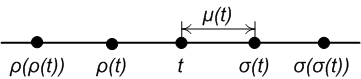
\includegraphics[width=0.4\paperwidth]{operators}
\end{figure}

\end{frame}

\begin{frame}
\frametitle{\subsecname}

La integración se define de modo que $\int_{t}^{s}f^{\Delta}\left(\tau\right)\Delta\tau=f\left(t\right)-f\left(s\right)$.

Si $\mathds{T}$ consiste únicamente de puntos aislados, entonces \[ f^{\Delta}\left(t\right)=\frac{f\left(\sigma\left(t\right)\right)-f\left(t\right)}{\mu\left(t\right)} \]

y

\[
\int_{a}^{b}f\left(t\right)\Delta t=
\begin{cases}
\sum_{t\in\left[a,b\right)\cap\mathds{T}}\mu\left(t\right)f\left(t\right),&\text{si }a<b.\\
0, & \text{si } a = b.\\
-\sum_{t\in\left[b,a\right)\cap\mathds{T}}\mu\left(t\right)f\left(t\right), & \text{si }a>b.
\end{cases}
\]
\end{frame}

%\subsubsection{Derivada fraccionaria}
\subsection{Módulo \texttt{timescale}}

{
	\usebackgroundtemplate{\centering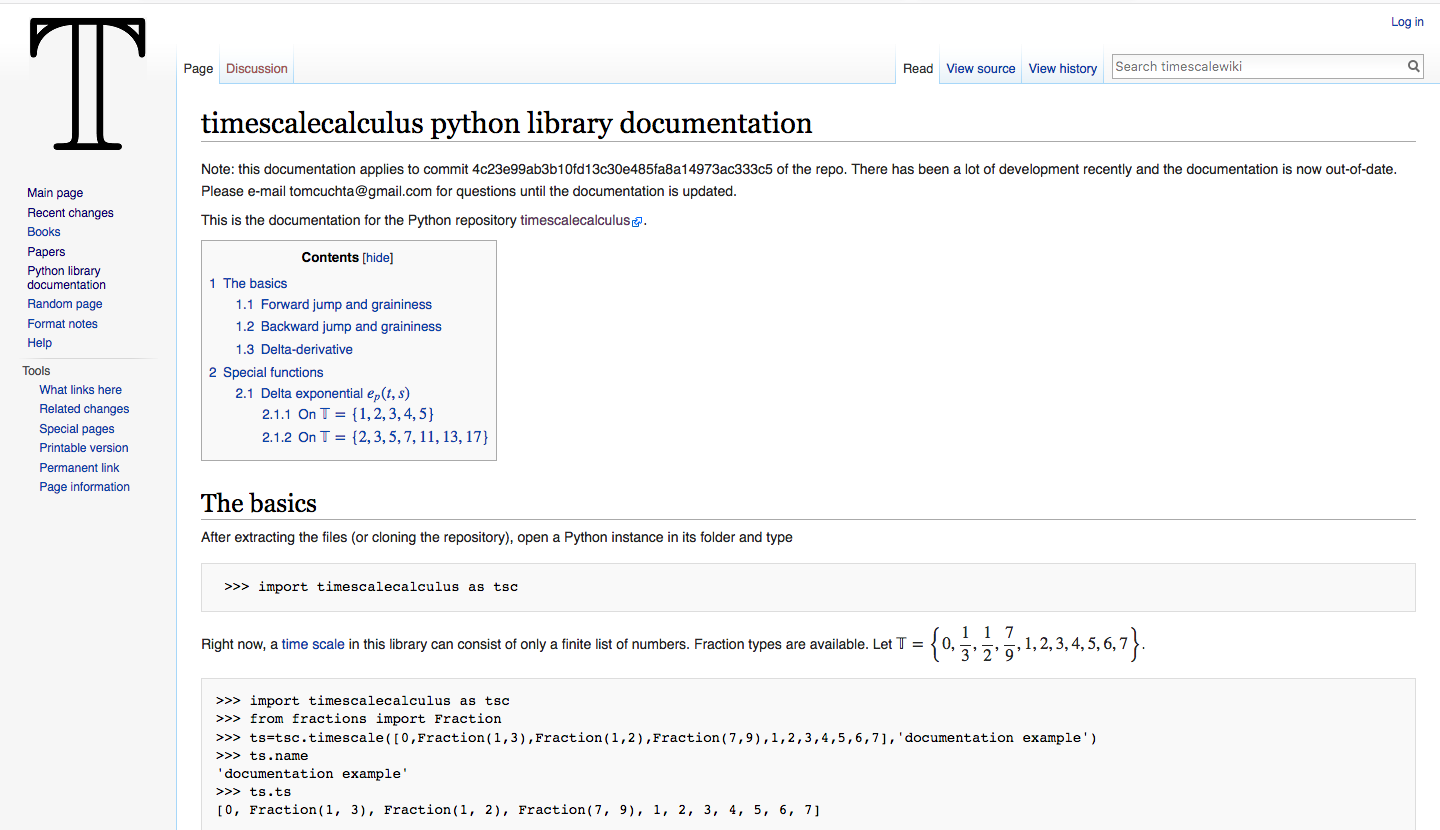
\includegraphics[width=\paperwidth]{doc}}
	\begin{frame}[plain]
	\end{frame}
}